%%%%%%%%%%%%%%%%%%%%%%%%%%%%%%%%%%%%%%%%%
% FRI Data Science_report LaTeX Template
% Version 1.0 (28/1/2020)
% 
% Jure Demšar (jure.demsar@fri.uni-lj.si)
%
% Based on MicromouseSymp article template by:
% Mathias Legrand (legrand.mathias@gmail.com) 
% With extensive modifications by:
% Antonio Valente (antonio.luis.valente@gmail.com)
%
% License:
% CC BY-NC-SA 3.0 (http://creativecommons.org/licenses/by-nc-sa/3.0/)
%
%%%%%%%%%%%%%%%%%%%%%%%%%%%%%%%%%%%%%%%%%


%----------------------------------------------------------------------------------------
%	PACKAGES AND OTHER DOCUMENT CONFIGURATIONS
%----------------------------------------------------------------------------------------
\documentclass[fleqn,moreauthors,10pt]{ds_report}
\usepackage[english]{babel}
\usepackage{comment}
\usepackage{numprint}
\usepackage{subcaption}

\graphicspath{{fig/}}



%----------------------------------------------------------------------------------------
%	ARTICLE INFORMATION
%----------------------------------------------------------------------------------------

% Header
\JournalInfo{FRI Natural language processing course 2023}

% Interim or final report
\Archive{Project report} 
%\Archive{Final report} 

% Article title
\PaperTitle{Project 3: Paraphrasing sentences} 

% Authors (student competitors) and their info
\Authors{Matjaž Zupančič Muc, Marko Novak, and Klemen Laznik}

% Advisors
\affiliation{\textit{Advisers: Slavko Žitnik}}

% Keywords
\Keywords{Sentence paraphrasing, Back-Translation, Paraphrase-Mining, Data Augmentation, Transformers, ParaScore.}
\newcommand{\keywordname}{Keywords}


%----------------------------------------------------------------------------------------
%	ABSTRACT
%----------------------------------------------------------------------------------------


\Abstract{
In this report we present 3 approaches to generating data for training paraphrasing models. The data is generated using backtranslation, by matching texts which have been translated by different human translators (i.e. movie subtitles), and by making simple, meaning-preserving augmentations on a corpus of sentences. We evaluate the obtained data based on accuracy, fluency, and diversity. We also explore parascore metric for automatic evaluation of the paraphrases. Finally, we train two T5 and BART models on the prepared dataset and evaluate their results usigng parascore.
}

%----------------------------------------------------------------------------------------

\begin{document}

% Makes all text pages the same height
\flushbottom

% Print the title and abstract box
\maketitle

% Removes page numbering from the first page
\thispagestyle{empty}

%----------------------------------------------------------------------------------------
%	ARTICLE CONTENTS
%----------------------------------------------------------------------------------------

\section*{Introduction}

\begin{comment}
These latex files are intended to serve as a the template for the NLP course at FRI.  The template is adapted from the FRI Data Science Project Competition. template  If you find mistakes in the template or have problems using it, please consult Jure Demšar (\href{mailto:jure.demsar@fri.uni-lj.si}{jure.demsar@fri.uni-lj.si}). In the Introduction section you should write about the relevance of your work (what is the purpose of the project, what will we solve) and about related work (what solutions for the problem already exist). Where appropriate, reference scientific work conducted by other researchers. For example, the work done by Demšar et al. \cite{Demsar2016BalancedMixture} is very important for our project. The abbreviation et al. is for et alia, which in latin means and others, we use this abbreviation when there are more than two authors of the work we are citing. If there are two authors (or if there is a single author) we just write down their surnames. For example, the work done by Demšar and Lebar Bajec \cite{Demsar2017LinguisticEvolution} is also important for successful completion of our project.
\end{comment}

Paraphrasing plays an important role in language understanding tasks, such as question answering, machine translation and semantic parsing. Additionally, it serves as a useful method for data augmentation. The goal of paraphrase generation is to produce alternative versions of a given sentence that feature different phrasing or structure, yet still accurately convey the original meaning. Creating high-quality paraphrases is a challenging problem in NLP, as it requires a deep understanding of the underlying semantics and syntax of the input sentence. In recent years, there has been a growing interest in using deep learning to automatically generate paraphrases.

%%%%%%%%%%%%%%%%%%%%%%%%%%%%%%%%%%%%%%%%%%%%%%%%%%%%%%%%%%%%%%%%%%%%
% Authors of \cite{federmann-etal-2019-multilingual} compare translation based paraphrase gathering using human (experts and non-experts), automatic and hybrid techniques. The automatic technique is based on back translation using a neural machine translation (NMT) model. They first translate a source sentence from one language to multiple target languages (i.e pivot languages) and than back to the original language. They found that NMT based paraphrases have a higher diversity compared to paraphrases written by human non experts, but NMT based paraphrases don't reach the adequacy or fluency level provided by expert paraphrases. They found that NMTs corrupt inputs such as slang and typing errors leading to bad paraphrases. They also found that NMTs struggle with negation, i.e NMTs tend to loose or add negation to a sentence. Finally they found that paraphrases generated by pivot languages which are closely related have a higher adequacy and fluency level, while paraphrases generated by pivot languages that are not closely related have higher diversity. They conclude that NMT based paraphrase generation is cheap and diverse, although NMTs produce less fluent outputs post editing could be used to improve the quality with little additional expenditure.

In \cite{federmann-etal-2019-multilingual}, the authors compare translation-based paraphrase gathering methods: human (experts and non-experts), automatic, and hybrid techniques. The automatic technique involves using a neural machine translation (NMT) model for back translation. NMT-based paraphrases are more diverse than those by non-experts but fall short in adequacy and fluency compared to expert paraphrases. NMT models struggle with inputs containing slang, typing errors, and negation, often leading to poor paraphrases. Paraphrases generated by closely related pivot languages show higher adequacy and fluency, while those from less related pivot languages offer more diversity. The authors conclude that NMT-based paraphrase generation is cost-effective and diverse, but post-editing can enhance quality with minimal additional effort. Existing paraphrase language models build on large encoder-decoder models. These models operate similarly to machine translation models, where the input is encoded and the decoder generates a new sequence. However, paraphrase models aim to produce output that differs from the input while preserving information, in contrast to machine translation models that generate similar representations of the input sentence. In {Paraphrase Generation: A Survey of the State of the Art}~\cite{zhou-bhat-2021-paraphrase}, the authors present several improvements on top of the encoder-decoder models, which are used by the current state-of-the-art models to achieve better results. \textbf{Attention} and \textbf{copy} mechanisms improve paraphrase generation by emphasising important information and determining whether to generate new tokens or copy from the input. To enhance diversity, \textbf{variational autoencoders} and \textbf{reinforcement learning} (RL) are used. RL, particularly with pretrained language models, enables unsupervised paraphrasing and addresses the training-evaluation mismatch (i.e we can directly optimise the metric of interest) RL-trained models also exhibit cross-lingual transfer without additional fine-tuning~\cite{DBLP:journals/corr/abs-2010-12885}. \textbf{Paraphrase evaluation} is a challenging problem, and existing metrics have limitations. In ~\cite{evaluation-metrics-in-paraphrase-generation}, the authors propose a new metric named ParaScore, which takes into account both semantic similarity and lexical divergence between the input sentence and candidate paraphrases. ParaScore is a reference-based metric and is defined as the maximum value between the semantic similarity of the candidate paraphrase to the reference paraphrase and the input sentence to the reference paraphrase, plus a weighted measure of lexical divergence. The authors also propose a reference-free version of ParaScore by removing the reference paraphrase from the metric. Authors conducted experiments on four datasets and compared ParaScore to several baselines, including BLEU, Rouge, METEOR, BERT-iBLEU, and iBLEU. The results show that ParaScore performs significantly better (i.e it achieves a higher correlation with human judgement of paraphrase quality) than all the other metrics on all the datasets and is more robust than other metrics. 

% well written, but i think we don't have the space :)
% Existing paraphrase generating language models build on large sequence-to-sequence / encoder-decoder language models. The general principle of those models is similar to models used in machine translations where the first part of the model creates an encoded representation of the input, and the decoder part generates a new sequence from the encoding. However, while machine translation models are trained to generate an output which closely represents the input sentence, for paraphrasing the output needs to differ from the input while maintaining information. \textbf{Attention} mechanism helps models emphasise the important information within the input. This information is passed to the decoder part of the model as an extra input vector. On the other hand, the \textbf{copy} mechanism helps determine whether to generate a new token or copy an input token at each step of decoding. This helps to improve the form of generated paraphrases, but limits the diversity of generated text. The two common approaches to improve the diversity of generated paraphrases are \textbf{variational autoencoders} (VAE) and \textbf{reinforcement learning} (RL); the benefit of using RL with a pretrained language model is that it doesn't require a large labelled dataset and can perform paraphrasing in unsupervised setting. RL also addresses the problem in the missmatch between the training goal and the evaluation metric. The networks are often trained to maximize the probability of generating the references paraphrases and that evaluated using metrics for paraphrase generation. RL can be trained to maximize the reward indicated as a desired evaluation metric. The models trained this way have also demonstrated the ability to perform cross-lingual transfer without additional finetuning~\cite{DBLP:journals/corr/abs-2010-12885}.

%%%%%%%%%%%%%%%%%%%%%%%%%%%%%%%%%%%%%%%%%%%%%%%%%%%%%%%%%%%%%%%%%%%%


% The ParaScore metric addresses some of the limitations of existing metrics, such as BLEU, which is a widely used metric but does not consider lexical divergence, and iBLEU, which considers lexical divergence but is sub-optimal. ParaScore provides a better evaluation of paraphrasing and has the potential to be used in applications such as text simplification and data augmentation.
%%%%%%%%%%%%%%%%%%%%%%%%%%%%%%%%%%%%%%%%%%%%%%%%%%%%%%%%%%%%%%%%%%%%


%% 

%------------------------------------------------

\section*{Methods}

% Given instructions, the proposed pipeline is as follows: Get an existing dataset (ccGigafida, ccKres, …). We might be able to use {Slovenian datasets for contextual synonym and antonym detection}~\cite{11356/1694} to obtain synonyms which could be used to generate paraphrased sentences from other corpora. Use Slovene NMTs to generate the dataset of paraphrases with first reference in mind.

 % Initial intuition of the dataset quality will be formed manually - human evaluation on smaller subgroups of data. Given the size of the data set, the end goal would be to find a consistent way to evaluate the quality of the entire data set, without introducing bias from any chosen method. Manual evaluation will include a few suggested metrics, e.g. similarity, clarity, fluency. We could evaluate the quality of the data set generated by NMTs using contextual similarity between original sentence and the paraphrased sentence. To do this we would embed the sentences using BERT and than compute the cosine similarity between the embeddings. We can use a readability score such as the Flesch Reading Ease score or the Gunning Fog Index to evaluate the clarity of the paraphrased sentences. To estimate the fluency we could use large language models such as BERT and GPT. BERT and GPT can be used to generate fluency scores based on the model's prediction of the likelihood of the sentence being a natural language sentence. Because fluency is closely related to grammatical correctness and syntax we check for grammar and syntax errors. We also though of using ParaScore (caution - this would require tuning to make useful, which is not suitable for this stage of the pipeline).

 % We'll train a baseline sequence to sequence T5 model on top of the generated dataset. We could use random pattern embeddings or add a diversity term to the loss function to increase the diversity of generated paraphrases. We also consider using a multilingual base model, as it would allow us to also use existing datasets from other languages and transfer that knowledge to Slovenian language.

% For training model evaluation, we turn to ParaScore. Given the width of the study~\cite{evaluation-metrics-in-paraphrase-generation}, we are lead to believe that for the task at hand - paraphrasing sentences, the existing metrics are insufficient in handling neither lexical diverging, nor semantic similarity simultaneously, which are both present. We should also be aware of potential drawback since we introduce a hyper-parameter in need of tuning. The idea behind using ParaScore is mainly to evaluate the quality of our paraphrasing model but are keen to use a similar approach to evaluate the NMTs output, which is the input - data for model training.

\subsection{Back Translation}

For the first dataset we took the sentences from {Training corpus SUK 1.0}~\cite{11356/1747}, which contains \numprint{48594} Slovenian sentences. We choose this corpus because it contains general, moderately-long sentences. For each sentence we then generated two paraphrased versions, first one by translating the original sentence to English and back to Slovene, and the second one by a two-stage backtranslation from Slovene to English, from English to German, and then back. This yielded good results both in terms of accuracy and diversity. However, as we used an online API to translate the sentences, we only generated a limited dataset due to the free API limitations.

This method is fast and generates good data without any additional effort from our side, so we can easily increase the dataset as we move forward and better determine how much data we need for model training.

% \textbf{TODO}: paraphrase mining dataset (how \& why ?)

\subsection{Paraphrase Mining}

The second dataset is constructed using a paraphrase-mining approach. We extract full sentences from two subtitle files of the same movie, each written by a different subtitle provider. For each sentence in the first subtitle file we find a corresponding sentence in the other subtitle file. The final dataset is a set of corresponding sentences. We found that if the two subtitle files are sampled at the same frame rate, we could somewhat align the subtitles and find the corresponding parts, however finding multiple sources of high quality subtitles both sampled at the same frame rate is not easy. As a result, we used a pre-trained BERT model trained on Croatian, Slovenian, and English corpora (~\cite{11356/1694}) to embed the sentences and discover corresponding sentences by calculating the pairwise cosine distance between the sentence embeddings. To decrease the number of false positive matches, we limited the comparison region of sentences. 

This approach can have several positive aspects. Multiple subtitle providers offer variations in translations, idiomatic expressions, and other nuances that can enrich the dataset. Generated paraphrases are potentially more human-like compared to fully automatic methods like back-translation. Bellow you can take a look at two example paraphrases (from the dataset) that we find to be of high quality.

\begin{scriptsize}
\begin{verbatim}
--------------------------------------------------------
"Ko te enkrat razglasijo za neprištevnega, potem vsako 
tvoje nadaljnje dejanje pripišejo tej norosti."  
"Ko si enkrat razglašen za norega, so vsa tvoja dejanja
zaznamovana s tem."

"Ali sta seznanjena z današnjim stanjem na področju 
mentalnega zdravljenja, gospoda?"
"Vesta, kakšno je današnje stanje na področju 
mentalnega zdravja?."
--------------------------------------------------------
\end{verbatim}
\end{scriptsize}

We should point out that the approach also has the following downsides: a subtitle author may include additional context (derived from the film plot) in their translations while the other may not. This can result in poor matches between sentences, since the context of the sentences may not align. As a result, the resulting paraphrase dataset may contain inaccuracies. Therefore the approach requires additional human effort to check the matched sentences, which can be time-consuming and costly. Despite the potential issues this approach can still be faster than writing human paraphrases from scratch.




% \textbf{TODO}: Future ideas (dataset of "incorrect-paraphrase examples", which model do we plan to train and why ?)
% We're looking at two sequence-to-sequence models for our paraphrasing model: BART and T5. Both architectures offer large pretrained models as well as multilingual variants, which could allow us to include examples from other languages in order to improve model performance. We'd also like to include some negative training examples, i.e. pairs of similar sentences that aren't paraphrases.
 

\subsection{Data Augmentation}

Due to the limited size of our training set, we undertake an exploration of different data augmentation techniques. The following transformations were utilised:

\begin{enumerate}
    \item \textbf{Paraphrase swapping}: Each paraphrase pair $\{p_1, p_2\}$ is used twice, enabling the model to learn mappings: $p_1 \rightarrow p_2$ and $p_2 \rightarrow p_1$. This effectively doubles the size of our dataset and introduces no additional noise.
    \item \textbf{Paraphrase duplication}: A dataset is constructed in the form of $\{p_i, p_i, 0\}$, where $p_i$ represents some sentence and $0$ indicates that the pair is not a paraphrase. This can be useful to penalise models for generating sentences which are too similar or have different meaning.
    \item \textbf{Synonym replacement}: Random synonyms in sentences are replaced to introduce lexical variations. Initially, we explored automatic techniques using WordNet, but found them to be too noisy. Instead, we manually replaced synonyms to ensure high-quality data augmentation. Hand replacement allows us to preserve the semantic similarity and grammatical compatibility. 
    
    % Using a text editor with a multiple word replacement functionality, we managed to generate $1013$ new paraphrase pairs in a relatively short period of time.

    % a subset of synonyms used: 
    %pogumen -> hraber
    %test -> preizkus
    %na prvi pogled -> na prvo žogo
    %posel -> biznis
    %rezultat -> izid
    %dejal / dejala -> rekel / rekla
    %zapisal — zabeležil
    %najpozneje -> najkasneje
    %sposobnost -> zmožnost
    %večino -> velik delež
    %simptomi -> znaki    
\end{enumerate}


\subsection{T5 Model}

T5 (Text-To-Text Transfer Transformer) is a transformer-based model typically used for translation and text summarization. We fine-tune the t5-sl-large model (\cite{ulvcar2022sequence}) on the task of paraphrase generation. For model evaluation, we turn to ParaScore. Given the width of the study~\cite{evaluation-metrics-in-paraphrase-generation}, we are lead to believe that for the task at hand - paraphrasing sentences, the existing metrics are insufficient in handling neither lexical diverging, nor semantic similarity simultaneously, which are both present. To compute the Parascore on Slovene sentences we used the crosloengual-bert model (\cite{ulcar-robnik2020finest}).

% We should also be aware of potential drawback since we introduce a hyper-parameter in need of tuning. The idea behind using ParaScore is mainly to evaluate the quality of our paraphrasing model but are keen to use a similar approach to evaluate the NMTs output, which is the input - data for model training.


% The model was trained with the following hyper-parameters: batch size $B=8$, learning rate $\alpha = 1e-4$ and weight decay $\gamma = 1.5e-4$, we trained the model with the AdamW optimiser, optimising the Cross Entropy (CE) Loss for $5$ epochs. Figure ~\ref{fig:t5_loss_aug_data} shows the CE loss on the train and validation set. 
%\begin{figure}[ht]\centering
%	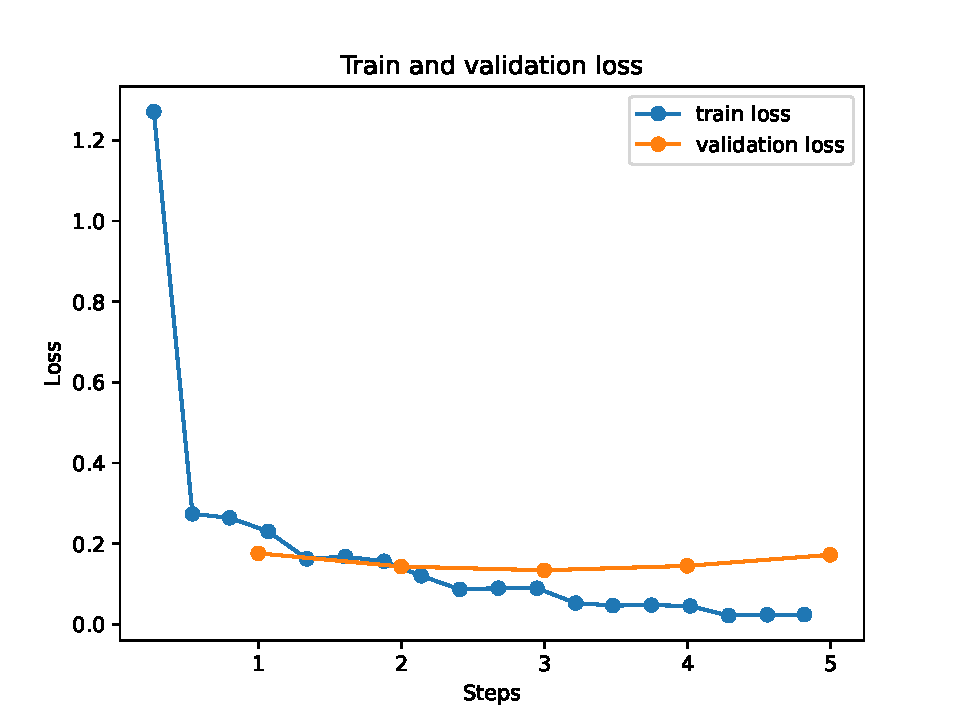
\includegraphics[width=\linewidth]{report/fig/t5_loss_aug_data.pdf}
%	\caption{}
%	\label{fig:t5_loss_aug_data}
%\end{figure}


% [\textbf{TODO}: Briefly describe the model]

\subsection{BART Model}

BART is a sequence-to-sequence model, which combines a bidirectional encoder over noisy or masked data with an auto-regressive decoder. When introduced, BART achieved state-of-the-art results for text summarisation~\cite{lewis2019bart}, as well as several other text-to-text tasks. Therefore we're interested to see how well it performs compared to the T5 model.





\begin{comment}
Use the Methods section to describe what you did an how you did it -- in what way did you prepare the data, what algorithms did you use, how did you test various solutions ... Provide all the required details for a reproduction of your work.Below are \LaTeX examples of some common elements that you will probably need when writing your report (e.g. figures, equations, lists, code examples ...).


\subsection*{Equations}

You can write equations inline, e.g. $\cos\pi=-1$, $E = m \cdot c^2$ and $\alpha$, or you can include them as separate objects. The Bayes’s rule is stated mathematically as:

\begin{equation}
	P(A|B) = \frac{P(B|A)P(A)}{P(B)},
	\label{eq:bayes}
\end{equation}

where $A$ and $B$ are some events. You can also reference it -- the equation \ref{eq:bayes} describes the Bayes's rule.

\subsection*{Lists}

We can insert numbered and bullet lists:

% the [noitemsep] option makes the list more compact
\begin{enumerate}[noitemsep]
	\item First item in the list.
	\item Second item in the list.
	\item Third item in the list.
\end{enumerate}

\begin{itemize}[noitemsep]
	\item First item in the list.
	\item Second item in the list.
	\item Third item in the list.
\end{itemize}

We can use the description environment to define or describe key terms and phrases.

\begin{description}
	\item[Word] What is a word?.
	\item[Concept] What is a concept?
	\item[Idea] What is an idea?
\end{description}


\subsection*{Random text}

This text is inserted only to make this template look more like a proper report. Lorem ipsum dolor sit amet, consectetur adipiscing elit. Etiam blandit dictum facilisis. Lorem ipsum dolor sit amet, consectetur adipiscing elit. Interdum et malesuada fames ac ante ipsum primis in faucibus. Etiam convallis tellus velit, quis ornare ipsum aliquam id. Maecenas tempus mauris sit amet libero elementum eleifend. Nulla nunc orci, consectetur non consequat ac, consequat non nisl. Aenean vitae dui nec ex fringilla malesuada. Proin elit libero, faucibus eget neque quis, condimentum laoreet urna. Etiam at nunc quis felis pulvinar dignissim. Phasellus turpis turpis, vestibulum eget imperdiet in, molestie eget neque. Curabitur quis ante sed nunc varius dictum non quis nisl. Donec nec lobortis velit. Ut cursus, libero efficitur dictum imperdiet, odio mi fermentum dui, id vulputate metus velit sit amet risus. Nulla vel volutpat elit. Mauris ex erat, pulvinar ac accumsan sit amet, ultrices sit amet turpis.

Phasellus in ligula nunc. Vivamus sem lorem, malesuada sed pretium quis, varius convallis lectus. Quisque in risus nec lectus lobortis gravida non a sem. Quisque et vestibulum sem, vel mollis dolor. Nullam ante ex, scelerisque ac efficitur vel, rhoncus quis lectus. Pellentesque scelerisque efficitur purus in faucibus. Maecenas vestibulum vulputate nisl sed vestibulum. Nullam varius turpis in hendrerit posuere.


\subsection*{Figures}

You can insert figures that span over the whole page, or over just a single column. The first one, \figurename~\ref{fig:column}, is an example of a figure that spans only across one of the two columns in the report.

\begin{figure}[ht]\centering
	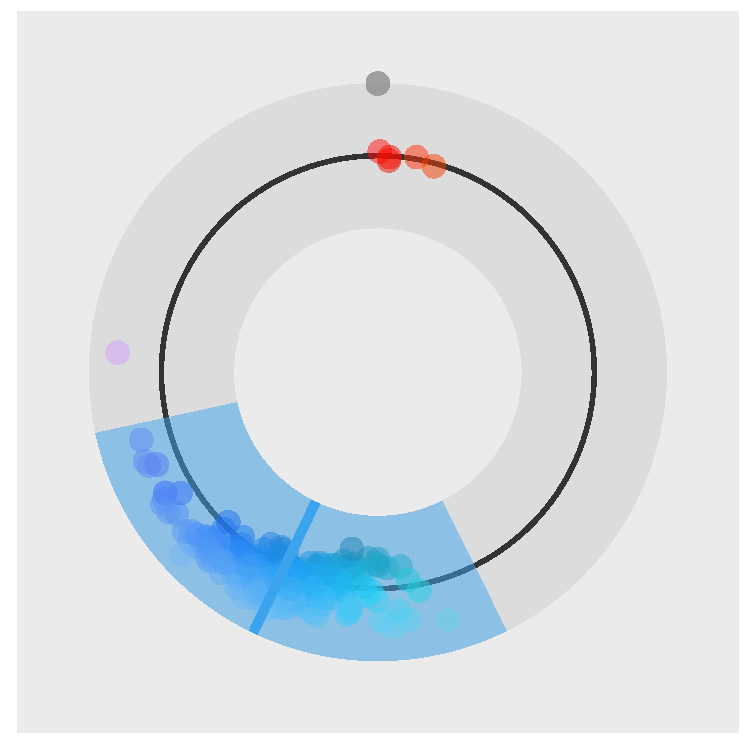
\includegraphics[width=\linewidth]{single_column.pdf}
	\caption{\textbf{A random visualization.} This is an example of a figure that spans only across one of the two columns.}
	\label{fig:column}
\end{figure}

On the other hand, \figurename~\ref{fig:whole} is an example of a figure that spans across the whole page (across both columns) of the report.

% \begin{figure*} makes the figure take up the entire width of the page
\begin{figure*}[ht]\centering
	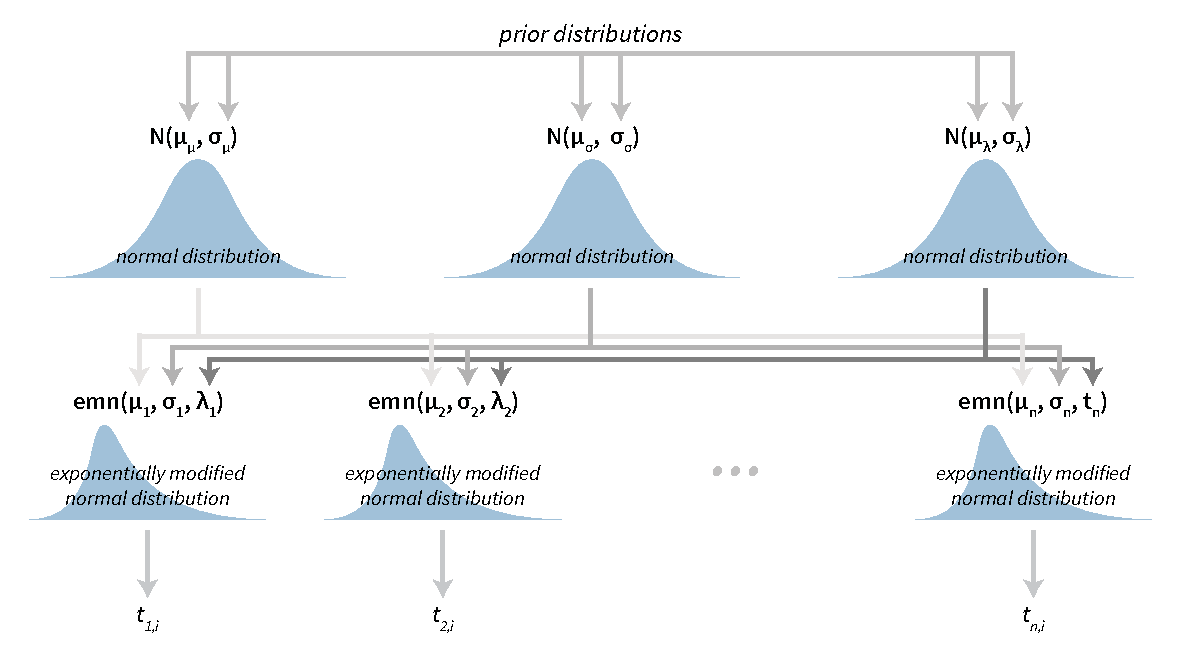
\includegraphics[width=\linewidth]{whole_page.pdf}
	\caption{\textbf{Visualization of a Bayesian hierarchical model.} This is an example of a figure that spans the whole width of the report.}
	\label{fig:whole}
\end{figure*}


\subsection*{Tables}

Use the table environment to insert tables.

\begin{table}[hbt]
	\caption{Table of grades.}
	\centering
	\begin{tabular}{l l | r}
		\toprule
		\multicolumn{2}{c}{Name}       \\
		\cmidrule(r){1-2}
		First name & Last Name & Grade \\
		\midrule
		John       & Doe       & $7.5$ \\
		Jane       & Doe       & $10$  \\
		Mike       & Smith     & $8$   \\
		\bottomrule
	\end{tabular}
	\label{tab:label}
\end{table}


\subsection*{Code examples}

You can also insert short code examples. You can specify them manually, or insert a whole file with code. Please avoid inserting long code snippets, advisors will have access to your repositories and can take a look at your code there. If necessary, you can use this technique to insert code (or pseudo code) of short algorithms that are crucial for the understanding of the manuscript.

\lstset{language=Python}
\lstset{caption={Insert code directly from a file.}}
\lstset{label={lst:code_file}}
\lstinputlisting[language=Python]{code/example.py}

\lstset{language=R}
\lstset{caption={Write the code you want to insert.}}
\lstset{label={lst:code_direct}}
\begin{lstlisting}
import(dplyr)
import(ggplot)

ggplot(diamonds,
	   aes(x=carat, y=price, color=cut)) +
  geom_point() +
  geom_smooth()
\end{lstlisting}

\end{comment}
%------------------------------------------------

\section*{Results}

\subsection{Dataset Evaluation}

 We evaluated the quality of 200 random paraphrase pairs generated using the paraphrase-mining technique and 100 paraphrase pairs generated using the back-translation technique. We assigned a score from 1 (poor) to 5 (excellent) for each of three metrics to each paraphrase pair.

\begin{enumerate}
    \item \textbf{Accuracy}: A measure of how well the paraphrase conveys the same meaning as the original text. 
    % A paraphrase that is accurate should capture the key ideas and information of the original text while maintaining the same overall meaning and context.

    \item \textbf{Fluency}: A measure of how well the paraphrase reads or sounds in the context of the original sentence or text. 
    % A paraphrase that is fluent should be grammatically correct, well-structured, and convey the same meaning as the original text, while also being easy to read or understand.

    \item \textbf{Diversity}: A measure of how different or unique the paraphrase is from the original text. 
    % A paraphrase that is diverse or original should convey the same meaning as the original text, but using different words or structures, and avoiding excessive copying or close similarity to the original text
\end{enumerate}

\begin{table}[!h]
\caption{Overall metric scoring results}
\begin{tabular}{lrr}
          & \multicolumn{1}{c}{\textbf{Back-translation}} & \multicolumn{1}{c}{\textbf{Paraphrase-mining}} \\
Accuracy  & $4.29 \pm 0.93$                                       & $4.12 \pm 1.10$                                              \\
Fluency   & $4.28 \pm 0.85$                                       & $4.17 \pm 1.05$                                              \\
Diversity & $3.31 \pm 1.22$                                       & $3.03 \pm 1.25$                             

\end{tabular}
\end{table}

The average \textbf{accuracy} score for the data-set is 4.29 (in case of back-translation), with a standard deviation of 0.93. The scores provided by the annotators indicate that the dataset generally contains accurate information, with an overall high level of correctness. The relatively small standard deviation suggests that there is a moderate level of agreement among the annotators regarding the accuracy of the dataset. On average, paraphrase-mining did provide a lower accuracy score and a larger deviation among the annotators.

The average \textbf{fluency} score for the dataset is 4.28 (in case of back-translation), with a standard deviation of 0.85. The scores indicate that the dataset generally exhibits a high level of fluency, meaning that the language used is smooth and natural-sounding. Similar to accuracy, the small standard deviation suggests a moderate level of agreement among the annotators in terms of fluency. When comparing both data acquisition methods, we can see the trend where back-translation tends to just about outperform paraphrase-mining. Better overall score and better coherency in human evaluation.

The average \textbf{diversity} score for the dataset is 3.31 (in case of back-translation), with a standard deviation of 1.22. The scores provided by the annotators indicate that the dataset has a moderate level of diversity, suggesting that it contains a reasonable variety of different examples or elements. The relatively larger standard deviation in this case implies that there might be some divergence in opinions among the annotators regarding the diversity of the dataset. It is important to note that many sentences contain the same content, which results in higher accuracy but lower diversity. Paraphrase-mining yields the biggest score difference in the ability to generate a diverse enough sentence.

High validity and reliability of measurements are crucial for providing meaningful and trustable results. To further explore and interpret the discrepancies in annotators scoring, we turn to Krippendorff's alpha coefficient. It is a reliability coefficient developed to measure the agreement among observers, coders, judges, raters, or measuring instruments drawing distinctions among typically unstructured phenomena or assign computable values to them. Krippendorff's alpha in contrast is based on the observed disagreement corrected for disagreement expected by chance. This leads to a range of -1 to 1 for both measures, where 1 indicates perfect agreement, 0 indicates no agreement beyond chance and negative values indicate inverse agreement.

\begin{table}[!h]
\caption{Krippendorff's alpha coefficient results}
\begin{tabular}{lrr}
          & \multicolumn{1}{c}{\textbf{Back-translation}} & \multicolumn{1}{c}{\textbf{Paraphrase-mining}} \\
Accuracy  & $0.44$                                       & $0.34$                                              \\
Fluency   & $0.36$                                       & $0.42$                                              \\
Diversity & $0.07$                                       & $0.12$                             

\end{tabular}
\end{table} 

Coefficient calculation only rewards the inputs where all annotators agree on the exact same value - category. The equation itself does not imply that data should be ordinal, and similar scores do not contribute positively to the outcome. This generality makes the scoring useful for any data input, but does provide worse results for big or small deviations. It is important to report both standard deviation and annotators agreements scores to interpret the human evaluation accordingly. All scores are skewed towards agreement, but are as close to randomness in case of paraphrase diversity.

\subsection{Model Evaluation}

% [\textbf{TODO}: Report evaluation metrics, display a subset of predictions, compare the approaches, models, etc.]

\subsubsection{T5-Base}


We trained the model on the original dataset (consisting of around $8000$ sentences) with the following hyper-parameters: batch size $B=8$, learning rate $\alpha = 1e-4$ and weight decay $\gamma = 1.5e-4$. We used the AdamW optimiser, and trained the model for $2$ epochs (after that the validation loss plateaus). The first row in Table ~\ref{tab:models-performance} shows the mean ref-based and ref-free parascore and the fraction of paraphrases which are identical to the input sentence. We can see that both the ref-based and ref-free parascore are high, however the copy fraction of $0.25$ is also relatively high. Figures ~\ref{fig:t5-parascore-hist} (a) and (b) display the histograms of ref-based parascore and ref-free parascore, we can see that majority of values are concentrated around the $0.95$ mark. 

\begin{figure}[ht]
    \centering
    \begin{subfigure}{0.45\linewidth} % Adjust the width as desired
        \centering
        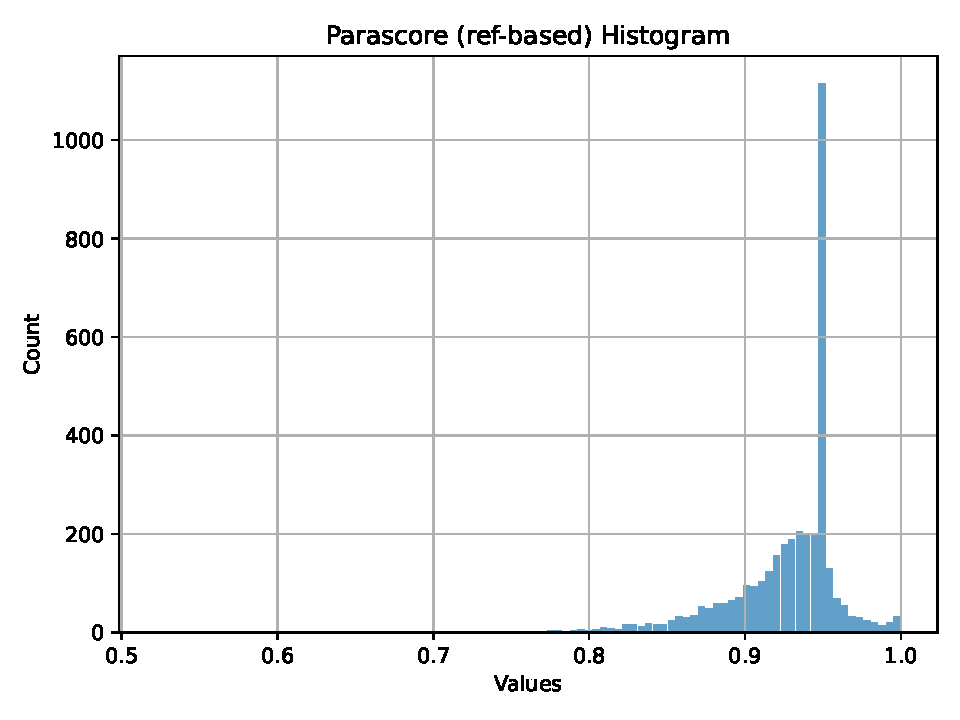
\includegraphics[width=\textwidth]{report/fig/t5-base-parascore-ref-based-hist.pdf}
        \caption{\textbf{Ref-based parascore}.}
        \label{fig:t5-base-parascore-ref-based-hist}
    \end{subfigure}
    \hfill % Add horizontal spacing between subfigures
    \begin{subfigure}{0.45\linewidth} % Adjust the width as desired
        \centering
        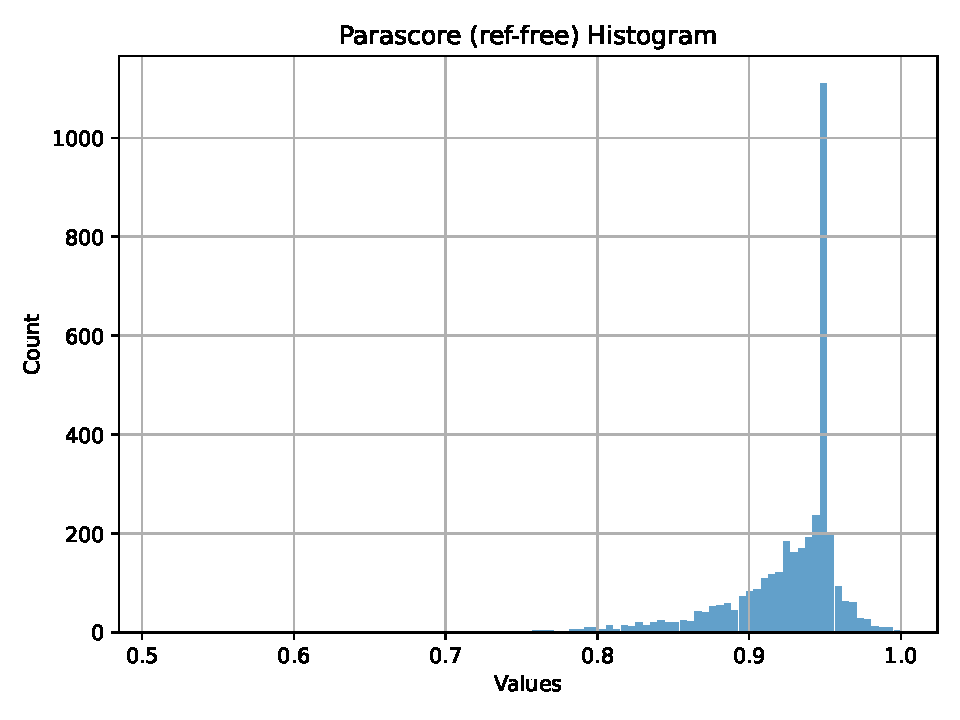
\includegraphics[width=\textwidth]{report/fig/t5-base-parascore-ref-free-hist.pdf}
        \caption{\textbf{Ref-free parascore}}
        \label{fig:t5-base-parascore-ref-free-hist}
    \end{subfigure}
    \caption{\textbf{Histograms of parascore values}. Parascore is computed on the test set using the finetuned \textbf{T5-Base} model.}
    \label{fig:t5-base-parascore-hist}
\end{figure}


After further investigation we found that most of the sentences with ref-based and ref-free parascore of $0.95$ actually correspond to copy paste paraphrases, this can be seen on Figure ~\ref{fig:t5-copy-paste-hist}. This implies that using only parascore to evaluate model performance is not enough and one should also compute at least the fraction of copy-pasted paraphrases.

\begin{figure}[ht]
    \centering
    \begin{subfigure}{0.45\linewidth} % Adjust the width as desired
        \centering
        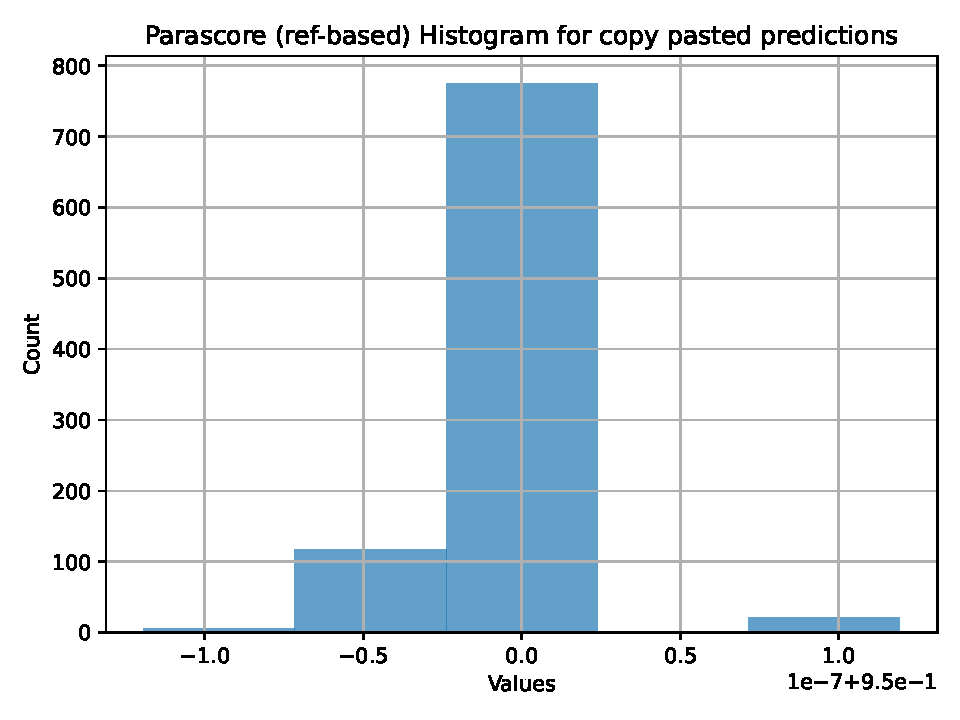
\includegraphics[width=\textwidth]{report/fig/t5-base-copy-preds-parascore-ref-based-hist.pdf}
        \caption{\textbf{Ref-based parascore}.}
        \label{fig:t5-aug-parascore-ref-based-hist}
    \end{subfigure}
    \hfill % Add horizontal spacing between subfigures
    \begin{subfigure}{0.45\linewidth} % Adjust the width as desired
        \centering
        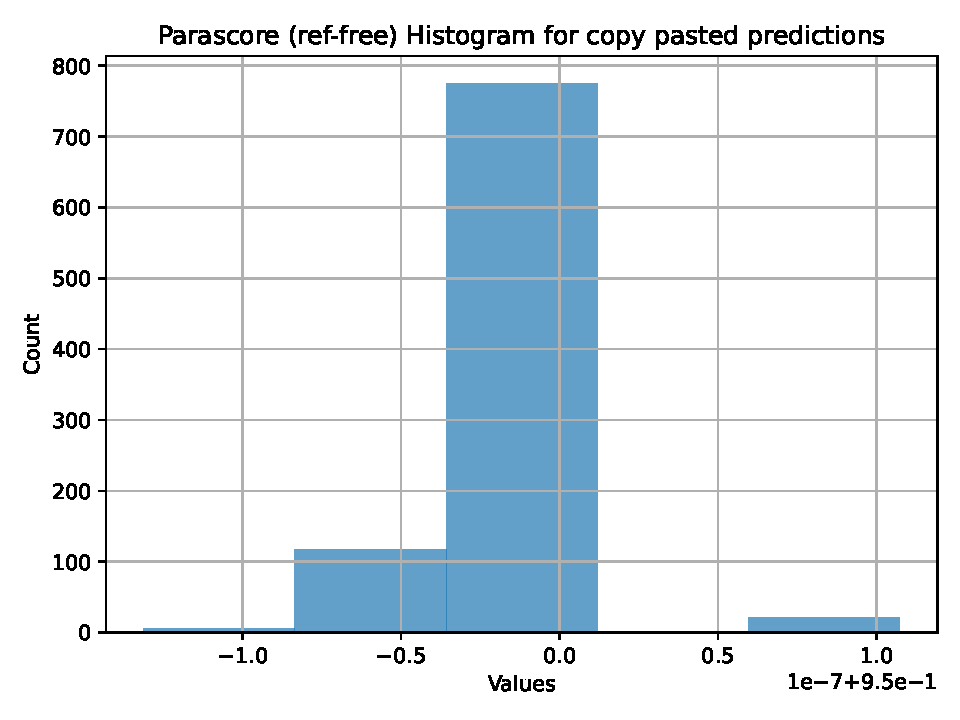
\includegraphics[width=\textwidth]{report/fig/t5-base-copy-preds-parascore-ref-free-hist.pdf}
        \caption{\textbf{Ref-free parascore}}
        \label{fig:t5-aug-parascore-ref-free-hist}
    \end{subfigure}
    \caption{\textbf{Histograms of parascore values for copy paste paraphrases}. Parascore is computed on the test set using the finetuned \textbf{T5-Base} model.}
    \label{fig:t5-copy-paste-hist}
\end{figure}


\subsubsection{T5-Aug}

Keeping all hyper-parameters constant, we train the model again this time on the augmented dataset (including swapped paraphrases and paraphrases with replaced synonyms). The augmented dataset consists of around $15000$ sentences. The model converged after $3$ epochs. The second row in Table ~\ref{tab:models-performance} shows the performance of the T5-Aug model, we can see that both the ref-based and ref-free parascore are lower than what we obtained with T5-Base, however the copy fraction of $0.11$ is also significantly lower, implying that T5-Aug model is much more creative when it comes to generating paraphrases. Figures ~\ref{fig:t5-parascore-hist} (a) and (b) display the histograms of ref-based parascore and ref-free parascore. We can see that the fraction of paraphrases with the score equal to $0.95$ is lower compared to what we observe on Figure ~\ref{fig:t5-base-parascore-hist}. Additionally, certain cases exhibit notably lower scores, reaching as low as $0.55$ for ref-based parascore and $0.39$ for ref-free parascore.

\begin{figure}[ht]
    \centering
    \begin{subfigure}{0.45\linewidth} % Adjust the width as desired
        \centering
        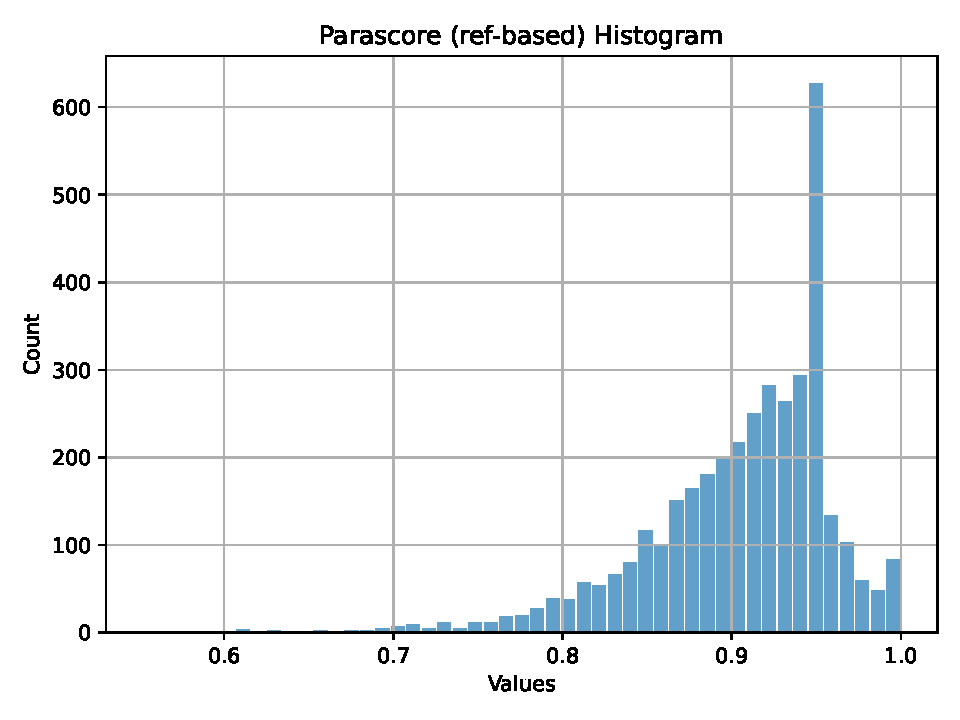
\includegraphics[width=\textwidth]{report/fig/t5-aug-parascore-ref-based-hist.pdf}
        \caption{\textbf{Ref-based parascore}.}
        \label{fig:t5-aug-parascore-ref-based-hist}
    \end{subfigure}
    \hfill % Add horizontal spacing between subfigures
    \begin{subfigure}{0.45\linewidth} % Adjust the width as desired
        \centering
        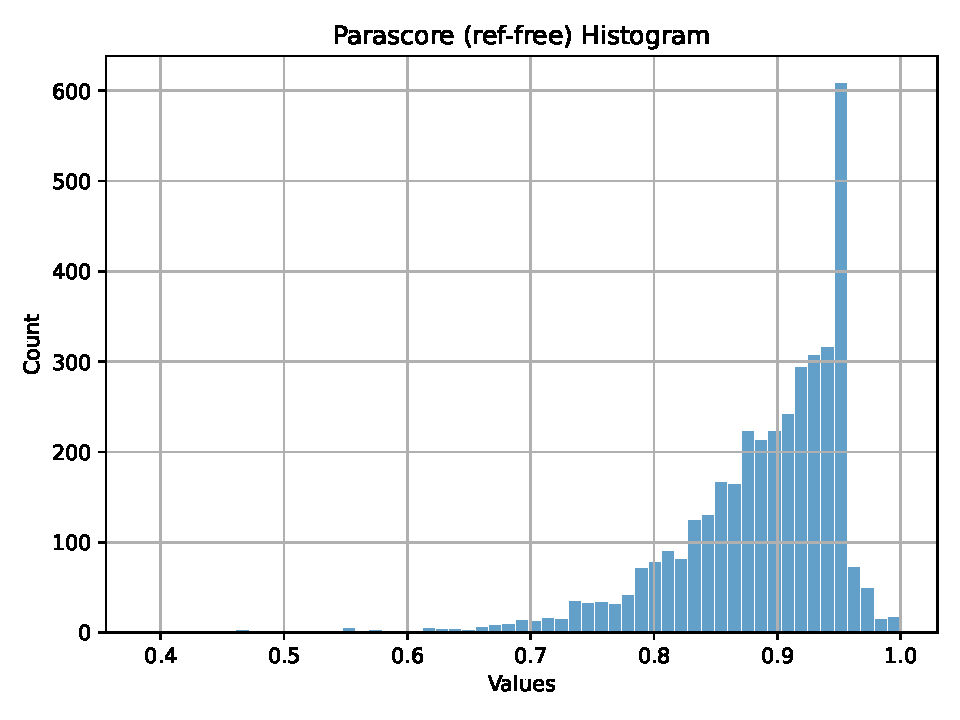
\includegraphics[width=\textwidth]{report/fig/t5-aug-parascore-ref-free-hist.pdf}
        \caption{\textbf{Ref-free parascore}}
        \label{fig:t5-aug-parascore-ref-free-hist}
    \end{subfigure}
    \caption{\textbf{Histograms of parascore values}. Parascore is computed on the test set using the finetuned \textbf{T5-Aug} model.}
    \label{fig:t5-parascore-hist}
\end{figure}

To gain a deeper understanding of the relationship between the parascore metric and the generated paraphrases, we examine a subset of predictions. Two illustrative examples are presented below, showcasing the paraphrase with the lowest ref-based parascore and the paraphrase with the highest ref-based parascore.
\begin{scriptsize}
\begin{verbatim}
--------------------------------------------------------
"O prodaji ne vedo"
"Prodaja ne ve, kaj prodaja"
ref-based-parascore=0.55

"Libijo je novembra 2009 z močno gospodarsko delegacijo 
obiskal predsednik vlade Borut Pahor." 
"Premier Borut Pahor je Libijo obiskal novembra 2009 
z močno poslovno delegacijo."
ref-based-parascore=1.0
--------------------------------------------------------
\end{verbatim}
\end{scriptsize}

Below are two representative examples that demonstrate the paraphrase with the lowest ref-free parascore and the paraphrase with the highest ref-free parascore.  The first example brings attention to another limitation of the parascore metric. Despite "Začuti žejo po krvi." being a valid paraphrase of "Željan je krvi." the ref-free-parascore equals only $0.39$. Interestingly the ref-based parascore for the reference:  "Čuti žejo po krvi." equals to $0.90$. This observation suggests that relying solely on the computation of a single parascore variation, whether it is ref-based or ref-free parascore, may not be sufficient. 

\begin{scriptsize}
\begin{verbatim}
--------------------------------------------------------
"Željan je krvi.",  
"Začuti žejo po krvi."
ref-free-parascore=0.39

"Slovenski in Bosanski organi naj bi do 19. septembra 
omogočili rešitev tega problema."
"Slovenski in bosanski organi naj bi omogočili rešitev
tega problema do 19. septembra."
ref-free-parascore=1.0
--------------------------------------------------------
\end{verbatim}

\end{scriptsize}

%\subsubsection{T5-All}
%[\textbf{TODO}: Figure out if we need this. Should we rather focus on something else?]

\subsubsection{BART-Base and BART-Aug}

We trained BART model using the same approach and data as with the T5 model. While the T5 model we used as a starting point has been trained on large Slovenian corpus, we didn't find an equivalent BART model, so we used a multilingual version of the model which includes Slovenian data. Compared to the T5 model, BART achieved a lower and more varying parascore, which is likely due to not being pretrained specifically for Slovenian language. However, it achieved a significantly lower copy factor, both on base and augmented data (\tablename~\ref{tab:models-performance}). Comparing the score distributions (\figurename~\ref{fig:t5-parascore-hist}, \figurename~\ref{fig:bart-aug-parascore-hist}), we can see BART had a much higher fraction of paraphrases with score below $0.7$, but at the same time also had a higher peak at $0.95$.

\begin{figure}[ht]
    \centering
    \begin{subfigure}{0.45\linewidth} % Adjust the width as desired
        \centering
        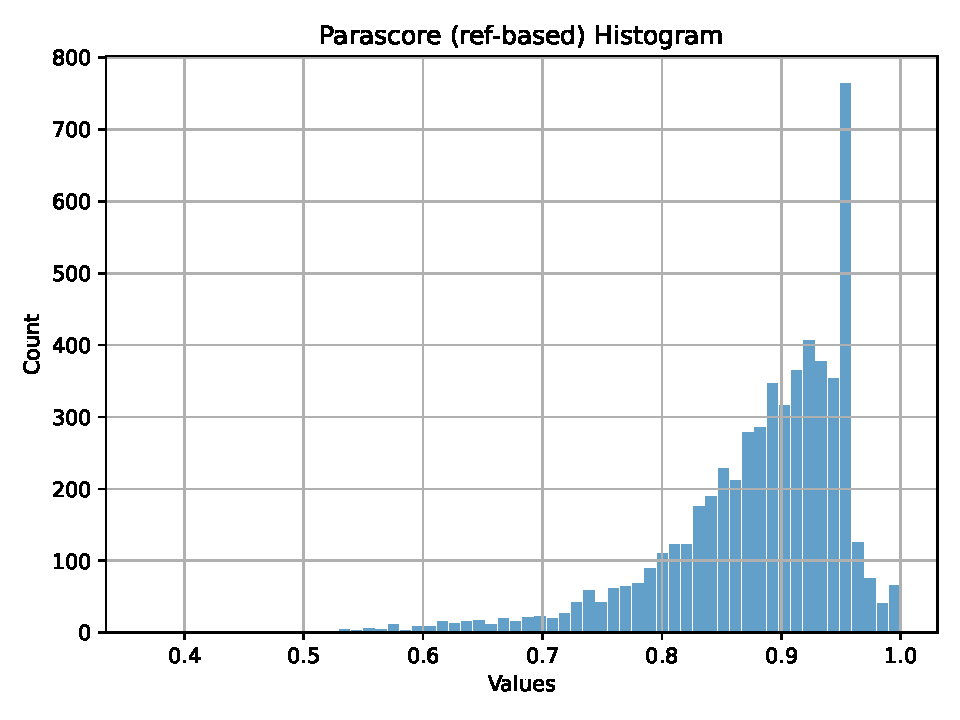
\includegraphics[width=\textwidth]{bart-aug-parascore-ref-based-hist.pdf}
        \caption{\textbf{Ref-based parascore}.}
        \label{fig:bart-aug-parascore-ref-based-hist}
    \end{subfigure}
    \hfill % Add horizontal spacing between subfigures
    \begin{subfigure}{0.45\linewidth} % Adjust the width as desired
        \centering
        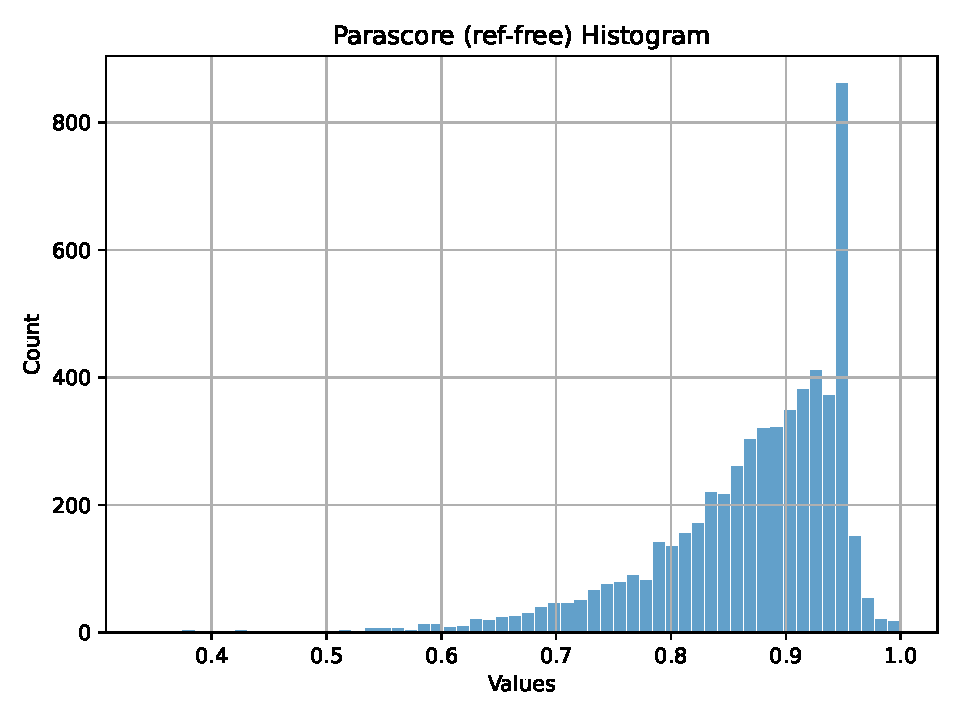
\includegraphics[width=\textwidth]{bart-aug-parascore-ref-free-hist.pdf}
        \caption{\textbf{Ref-free parascore}}
        \label{fig:bart-aug-parascore-ref-free-hist}
    \end{subfigure}
    \caption{\textbf{Histograms of parascore values}. Parascore is computed on the test set using the finetuned \textbf{BART-Aug} model.}
    \label{fig:bart-aug-parascore-hist}
\end{figure}

% \subsubsection{BART-Aug}

%\subsubsection{BART-All}
%[\textbf{TODO}: Figure out if we need this. Should we rather focus on something else?]

\begin{table}[!h]
\centering
\caption{Performance of all models on the test set. Columns \textbf{Para-ref} and \textbf{Para-ref-free} denote ref-based and ref-free parascore, while column \textbf{Copy Frac.} denotes the fraction of paraphrases that are identical to the source sentence.}
\begin{tabular}{lrrr}
\textbf{Model} & \textbf{Para-ref} & \textbf{Para-ref-free} & \textbf{Copy Frac.}\\ \hline
T5-Base & $0.91 \pm 0.043$ & $0.93 \pm 0.04$ & $0.25$ \\
T5-Aug & $0.91 \pm 0.056$ & $0.88 \pm 0.066$ & $0.11$ \\
% T5-All & 0 & 0 & 0 \\
BART-Base & $0.90 \pm 0.066$ & $0.88 \pm 0.073$ & $0.15$ \\
BART-Aug & $0.88 \pm 0.078$ & $0.87 \pm 0.084$ & $0.09$ \\ \hline
% BART-All & 0 & 0 & 0 \\ \hline
\end{tabular}
\label{tab:models-performance}
\end{table}


\subsection{Exploring Encoder-Decoder Attention}
% [\textbf{TODO}: Visualise encoder-decoder attention maps, try to find interesting examples and interpret them.]

In this section, our aim is to explain the extent to which we can comprehend the behaviour of the model. To achieve this, we intentionally create a relatively complex paraphrase and examine the encoder-decoder attention maps of the fine-tuned T5-Aug model. Our objective is to determine whether the model possesses the capability to establish the same connections that we, as human writers, made during the paraphrase composition process. As depicted in Figure ~\ref{fig:t5-sen1-cross-attention}, the cross-attention illustrates the relationship between the paraphrase (left column) and the source sentence (right column). Notably, on the left plot, we observe robust attention connections between words such as: "vodstvo-vlada," "implementiralo-sprejela," "strategije-ukrepe," and "napredka-razvoja." We should note that these synonymic connections are not trivial, as their establishment necessitates the incorporation of the entire sentence context. This observation highlights the model's ability to grasp the contextual nuances and capture the intricate dependencies required to effectively recognise and generate appropriate paraphrases. On the second plot, we observe an even more contextually driven connection formed by the model, i.e when encoding the word "okolje," the model attends to words like "zmanjšanje ogljičnega odtisa."

% In the context of paraphrase generation using the T5 model, the cross-attention provides valuable information about the model's ability to establish meaningful connections between different parts of the input and output sequences. It reveals how the model attends to specific words or phrases in the source sentence while generating the paraphrase. By examining the cross-attention patterns, we can understand which parts of the original sentence are considered important or influential in producing the paraphrased output.

%\begin{footnotesize}
%\begin{verbatim}
%"Glavni namen te raziskave je bil 
%ugotoviti povezave med prehrano in 
%psihičnim blagostanjem pri mladostnikih."
%"Cilj te študije je bil 
%identificirati korelacije med prehrano
%in duševnim zdravjem mladostnikov"
%\end{verbatim}
%\end{footnotesize}

%\begin{footnotesize}
%\begin{verbatim}
%"Vodstvo je implementiralo strategije 
%s ciljem spodbujanja trajnostnega 
%napredka ter zmanjšanja negativnega 
%vpliva na okolje v obliki ogljičnega odtisa."
%"Vlada je sprejela ukrepe za 
%spodbujanje trajnostnega razvoja 
%in zmanjšanje ogljičnega odtisa."
%\end{verbatim}
%\end{footnotesize}

\begin{figure}[ht]
    \centering
    \begin{subfigure}{0.45\linewidth} % Adjust the width as desired
        \centering
        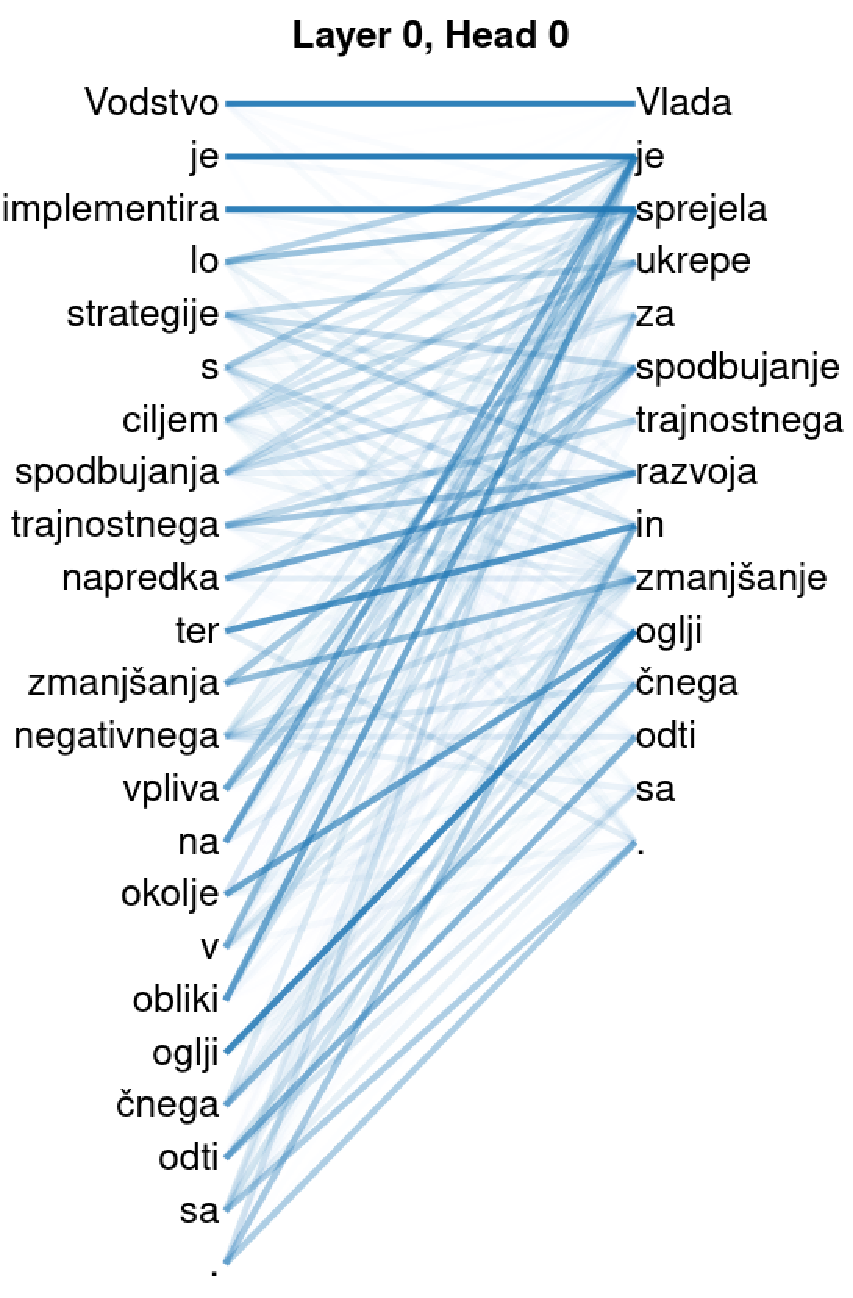
\includegraphics[width=\textwidth]{report/fig/t5-sen1-conn1.pdf}
        \label{fig:t5-sen1-conn1}
    \end{subfigure}
    \hfill % Add horizontal spacing between subfigures
    \begin{subfigure}{0.45\linewidth} % Adjust the width as desired
        \centering
        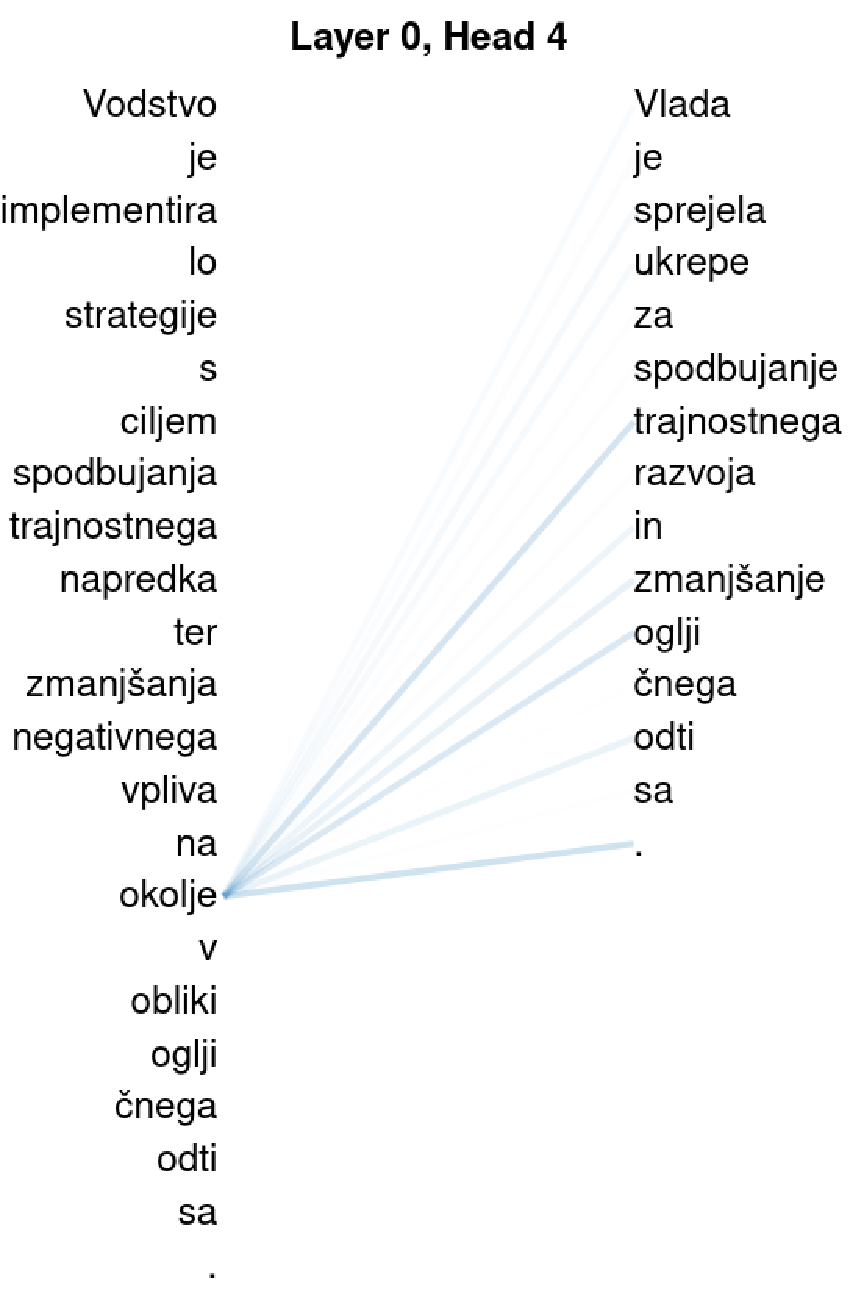
\includegraphics[width=\textwidth]{report/fig/t5-sen1-conn2.pdf}
        \label{fig:t5-sen1-conn2}
    \end{subfigure}
    \caption{\textbf{Encoder-Decoder Attention} paraphrased sentence (left column), original sentence (right column)}
    \label{fig:t5-sen1-cross-attention}
\end{figure}



\subsection{Correlation Between ParaScore and Human Judgement}

Given completed evaluation using automated computation model Parascore, we've already covered the obvious pitfalls when occurring paraphrased sentences which are just duplicates. The algorithm converges to a value of 0.95, and rarely exceeds that value. This brings up an inherent problem, where human evaluation punishes diversity by giving a low score, as opposed to parascore which provides the best scores exactly on duplicate sentences. We could be weighing individual metrics by some agreement, but the point of paraphrasing is to provide a different form of a sentence.

\begin{figure}[ht]
    \centering
    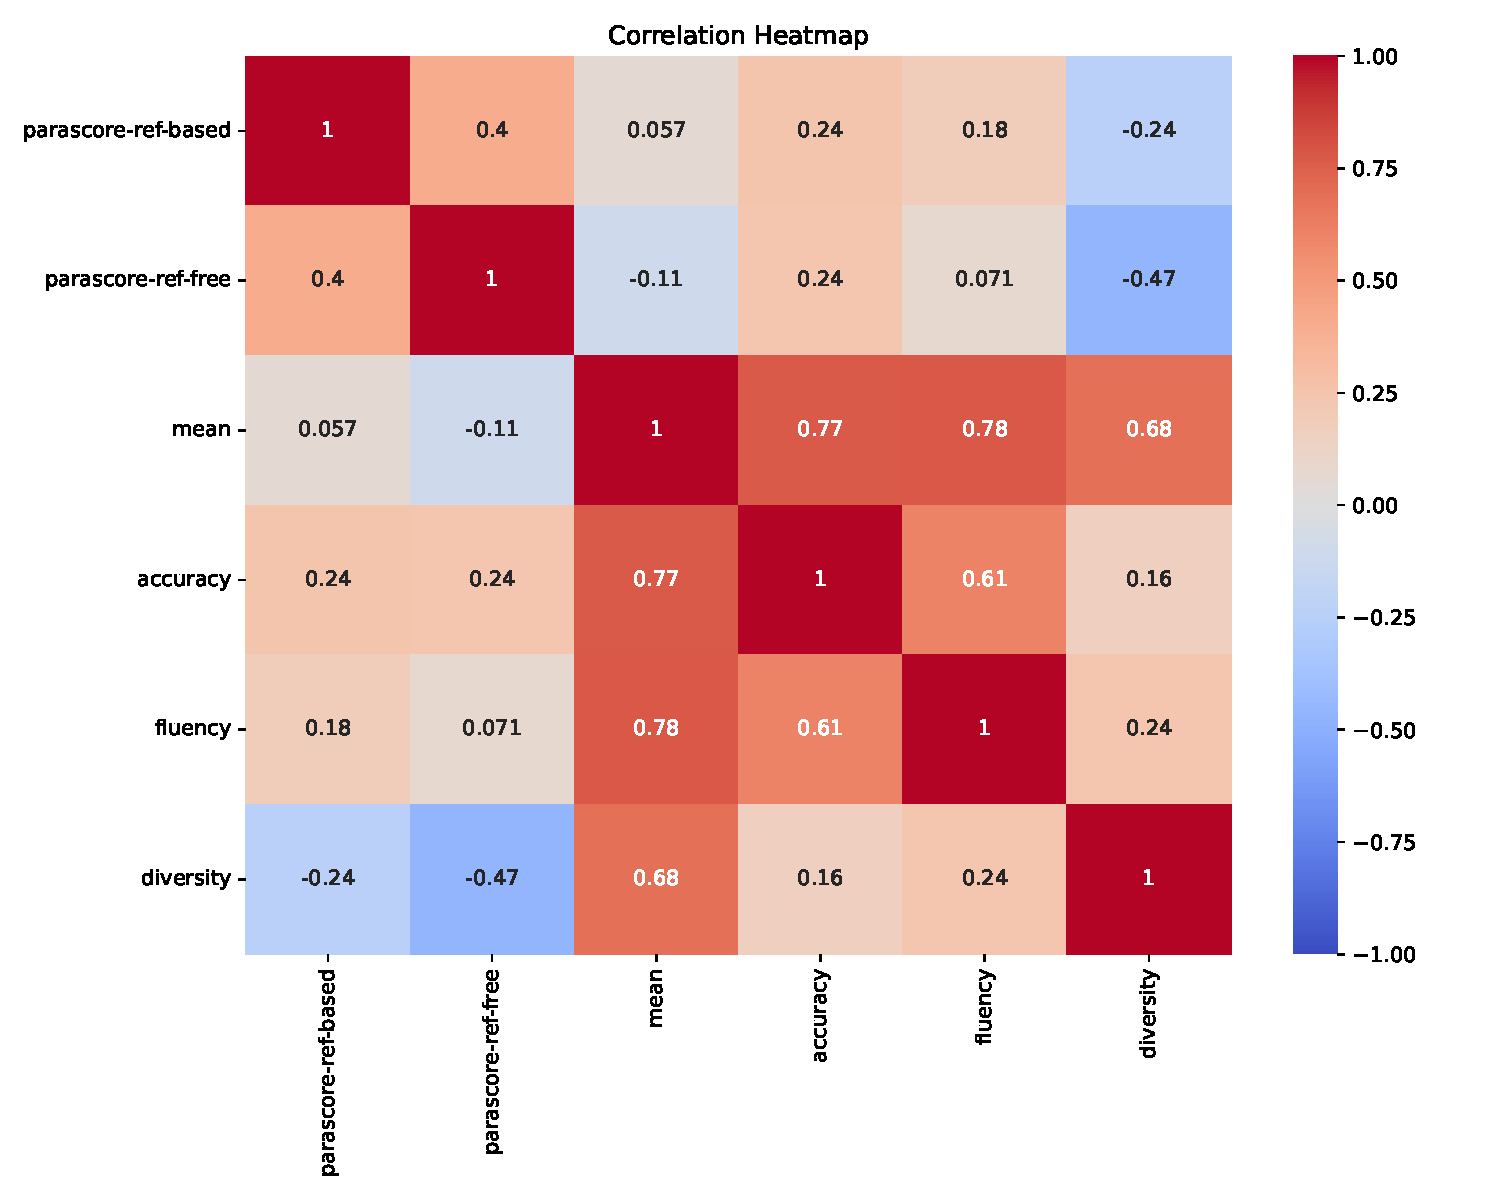
\includegraphics[width=0.45\textwidth]{report/fig/corr_heatmap.pdf}
    \caption{\textbf{Correlation heat map} among human evaluation using three metrics (accuracy, fluency and diversity) and both parascores - reference and non reference based}
    \label{fig:corr-heatmap}
\end{figure}

To further understand the correlation of human evaluation and parasocre on model predictions, we've allocated one annotator to evaluate additional 40 paraphrases in the same manner as in data set annotation. A table with all the human evaluated scores and both parascores is compared to find some correlation, to check for validity of automated evaluation of paraphrase quality.

As mentioned throughout parascore analysis, there is a greatly negative correlation between the parascores and diversity. This is caused by parascore giving relatively maximal scores on duplicated and the minimal score from a human annotator. What is also expected is that although the reference based and non reference based parascores are different, they are next best correlated amongst the human evaluation. To further break down the overall mean scores for human evaluation, it would seem that mean score is completely random when compared to any of the parascores. This is the exact reason we checked for individual metric, which show that mean correlation is close to zero because we combine the higher accuracy correlation and negative diversity correlation.

Going back to the Parascore introductory article, it is not providing one of the main conclusions, which is to punish low diversity accordingly. It does though focus on semantics, which is captured with accuracy, and lexical diversity. We've proven that accuracy is scored in a correlated fashion, but the diversity is scored inversely. Although the human evaluation pool is rather small, it is enough to see trends in validity of automated paraphrase scoring.

\begin{comment}


Use the results section to present the final results of your work. Present the results in a objective and scientific fashion. Use visualisations to convey your results in a clear and efficient manner. When comparing results between various techniques use appropriate statistical methodology.

\subsection*{More random text}

This text is inserted only to make this template look more like a proper report. Lorem ipsum dolor sit amet, consectetur adipiscing elit. Etiam blandit dictum facilisis. Lorem ipsum dolor sit amet, consectetur adipiscing elit. Interdum et malesuada fames ac ante ipsum primis in faucibus. Etiam convallis tellus velit, quis ornare ipsum aliquam id. Maecenas tempus mauris sit amet libero elementum eleifend. Nulla nunc orci, consectetur non consequat ac, consequat non nisl. Aenean vitae dui nec ex fringilla malesuada. Proin elit libero, faucibus eget neque quis, condimentum laoreet urna. Etiam at nunc quis felis pulvinar dignissim. Phasellus turpis turpis, vestibulum eget imperdiet in, molestie eget neque. Curabitur quis ante sed nunc varius dictum non quis nisl. Donec nec lobortis velit. Ut cursus, libero efficitur dictum imperdiet, odio mi fermentum dui, id vulputate metus velit sit amet risus. Nulla vel volutpat elit. Mauris ex erat, pulvinar ac accumsan sit amet, ultrices sit amet turpis.

Phasellus in ligula nunc. Vivamus sem lorem, malesuada sed pretium quis, varius convallis lectus. Quisque in risus nec lectus lobortis gravida non a sem. Quisque et vestibulum sem, vel mollis dolor. Nullam ante ex, scelerisque ac efficitur vel, rhoncus quis lectus. Pellentesque scelerisque efficitur purus in faucibus. Maecenas vestibulum vulputate nisl sed vestibulum. Nullam varius turpis in hendrerit posuere.

Nulla rhoncus tortor eget ipsum commodo lacinia sit amet eu urna. Cras maximus leo mauris, ac congue eros sollicitudin ac. Integer vel erat varius, scelerisque orci eu, tristique purus. Proin id leo quis ante pharetra suscipit et non magna. Morbi in volutpat erat. Vivamus sit amet libero eu lacus pulvinar pharetra sed at felis. Vivamus non nibh a orci viverra rhoncus sit amet ullamcorper sem. Ut nec tempor dui. Aliquam convallis vitae nisi ac volutpat. Nam accumsan, erat eget faucibus commodo, ligula dui cursus nisi, at laoreet odio augue id eros. Curabitur quis tellus eget nunc ornare auctor.
\end{comment}

%------------------------------------------------

\section*{Discussion}

%[\textbf{TODO}: Add a short comment for the remaining methods / contributions.]

The \textbf{Back Translation} method contributed to the majority of our dataset. We believe that utilising the same sentence twice, once to generate a paraphrase with \textit{sl $\rightarrow$ en $\rightarrow$ sl}  translation and the another paraphrase using \textit{sl $\rightarrow$ en $\rightarrow$ de $\rightarrow$ en $\rightarrow$ sl}  was a great way utilising the original set of sentences. Additionally this approach may have prevented the model to learn copy-pasting, as we provided it with multiple possible paraphrases of the original sentence. The \textbf{Paraphrase-Mining} approach using movie translations was intriguing and novel in our understanding. It yielded a small collection of human-like paraphrases, however, the manual filtering required for matching paraphrases proved to be time-consuming, limiting the size of the generated dataset. We have shown that the proposed \textbf{data-augmentation techniques} are effective at increasing the size, and diversity of the dataset, and thus yield better performing models. We found our \textbf{experiment on encoder-decoder attention} to be intriguing as it provided some insights into the connections made by the model during paraphrase generation. However, we acknowledge that our small-scale experiment cannot fully elucidate the inner workings of the model. 

To be fair, we cannot provide a guarantee that our solution surpasses the performance of the back-translation method. We also believe that the primary purpose of paraphrases generated through automatic techniques should be to expand the dataset size, rather than serving as the fundamental basis of the system. To achieve a system that surpasses the performance of the backtranslation technique, we advocate for the manual correction and validation of paraphrases generated automatically. Furthermore, the utilisation of a substantial collection of high-quality human-written paraphrases would significantly enhance the system's strength and effectiveness. In hindsight, if we had the opportunity to start from scratch, we would prioritise the creation of a vast paraphrase dataset using models such as GPT-3.5. By leveraging the language comprehension capabilities of these advanced (and expansive) models, we could engineer a more robust and cost-effective solution.


\begin{comment}
Use the Discussion section to objectively evaluate your work, do not just put praise on everything you did, be critical and exposes flaws and weaknesses of your solution. You can also explain what you would do differently if you would be able to start again and what upgrades could be done on the project in the future.
\end{comment}


%------------------------------------------------

\section*{Acknowledgments}

\begin{comment}
Here you can thank other persons (advisors, colleagues ...) that contributed to the successful completion of your project.
\end{comment}

%----------------------------------------------------------------------------------------
%	REFERENCE LIST
%----------------------------------------------------------------------------------------

\bibliographystyle{unsrt}
\bibliography{report}


\end{document}
